\chapter{Proyecciones Cartogr\'aficas}
\label{sec:proyecciones.cartograficos}


\begin{figure}[!htb]
  \centering
  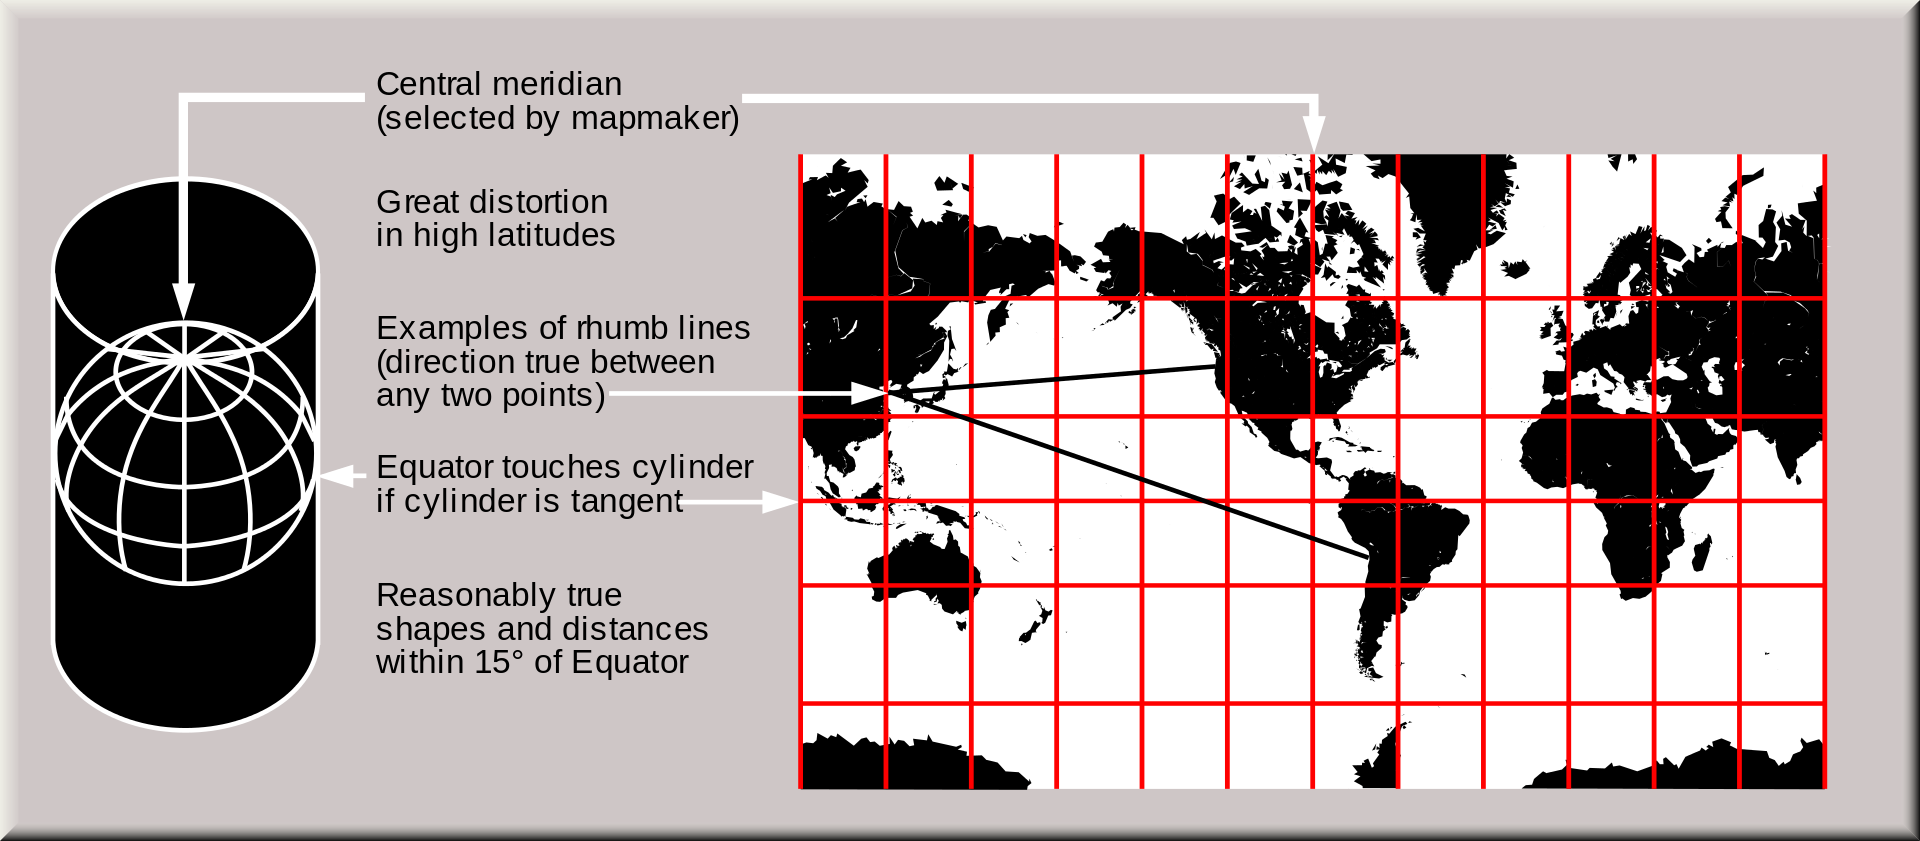
\includegraphics[width=\textwidth]{06.radionavegacion/Imagenes/proyeccion_mercator.png}
  \caption{\centering Sistema de proyecci\'on  Mercator, \\{\scriptsize Fuente \url{https://es.wikipedia.org/wiki/Proyecci%C3%B3n_de_Mercator#/media/Archivo:Usgs_map_mercator.svg}}}
  \label{fig:sistema.proyeccion.mercator}
\end{figure}



El \textbf{Sistema de Coordenadas Universal Transversal de Mercator} \ac{UTM} est\'a basado en un tipo de \gls{proyeccion-cartografica} denominada \emph{proyecci\'on geogr\'afica transversal de Mercator}, tangente a un meridiano. Las magnitudes en el sistema \ac{UTM} se expresan en metros al nivel del mar, que es la base de la proyecci\'on del elipsoide de referencia.

El sistema de coordenadas \ac{UTM} fue desarrollado por el Cuerpo de Ingenieros del Ejército de los Estados Unidos en la década de 1940. El sistema se basó en un modelo elipsoidal de la Tierra, emple\'andose el elipsoide de Clarke de 1866 para el territorio de los 48 estados contiguos. Para el resto del mundo, incluidos Alaska y Hawai, se usó el Elipsoide Internacional. Actualmente se usa el elipsoide WGS84 como modelo de base para el sistema de coordenadas \ac{UTM}.

Anteriormente al desarrollo del sistema de coordenadas \ac{UTM} varios países europeos ya habían experimentado la utilidad de mapas cuadriculados en proyección conforme, al cartografiar sus territorios en el período de entreguerras. El cálculo de distancias entre dos puntos con esos mapas sobre el terreno se hacía más fácil usando el teorema de Pitágoras, al contrario que con las fórmulas trigonométricas que había que emplear con los mapas referenciados en longitud y latitud. En los años de post-guerra estos conceptos se extendieron al sistema de coordenadas basado en las proyecciones \ac{UTM} y Estereográfica Polar Universal, que es un sistema cartográfico mundial basado en cuadrícula recta.

La Proyección Transversa de Mercator es una variante de la Proyección de Mercator que fue desarrollada por el geógrafo flamenco Gerardus Mercator en 1569. Esta proyección es conforme, es decir, que conserva los ángulos y casi no distorsiona las formas pero inevitablemente sí lo hace con distancias y áreas. El sistema \ac{UTM} implica el uso de escalas no lineales para las coordenadas X e Y (longitud y latitud cartográficas) para asegurar que el mapa proyectado resulte conforme.

\begin{figure}[!htb]
  \centering
  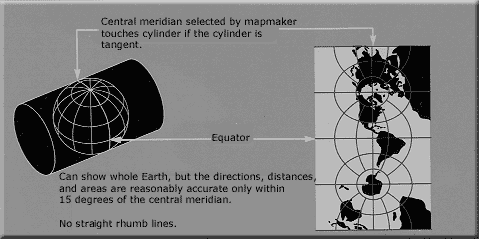
\includegraphics[width=\textwidth]{06.radionavegacion/Imagenes/Usgs_map_traverse_mercator.png}
  \caption{\centering Sistema de proyecci\'on transversa Mercator, \\{\scriptsize Fuente \url{https://commons.wikimedia.org/wiki/File:Usgs_map_traverse_mercator.PNG}}}
  \label{fig:sistema.proyeccion.transversa.mercator}
\end{figure}

La UTM es una proyección cilíndrica conforme. El factor de escala en la dirección del paralelo y en la dirección del meridiano son iguales (h = k). Las líneas loxodrómicas se representan como líneas rectas sobre el mapa. Los meridianos se proyectan sobre el plano con una separación proporcional a la del modelo, así hay equidistancia entre ellos. Sin embargo los paralelos se van separando a medida que nos alejamos del Ecuador, por lo que al llegar al polo las deformaciones serán infinitas. Por eso sólo se representa la región entre los paralelos 84ºN y 80ºS. Además es una proyección compuesta; la esfera se representa en trozos, no entera. Para ello se divide la Tierra en husos de 6º de longitud cada uno, mediante el artificio de Tyson .

La proyección UTM tiene la ventaja de que ningún punto está demasiado alejado del meridiano central de su zona, por lo que las distorsiones son pequeñas. Pero esto se consigue al coste de la discontinuidad: un punto en el límite de la zona se proyecta en coordenadas distintas propias de cada Huso.

Para evitar estas discontinuidades, a veces se extienden las zonas, para que el meridiano tangente sea el mismo. Esto permite mapas continuos casi compatibles con los estándar. Sin embargo, en los límites de esas zonas, las distorsiones son mayores que en las zonas estándar.

\begin{itemize}
	\item \textbf{  Husos UTM:}  Se divide la Tierra en 60 husos de 6º de longitud, la zona de
  proyección de la UTM se define entre los paralelos 80º S y 84º
  N. Cada huso se numera con un número entre el 1 y el 60, estando el
  primer huso limitado entre las longitudes 180° y 174° W y centrado
  en el meridiano 177º W. Cada huso tiene asignado un meridiano
  central, que es donde se sitúa el origen de coordenadas, junto con
  el ecuador. Los husos se numeran en orden ascendente hacia el
  este. Por ejemplo, la Península Ibérica está situada en los husos
  29, 30 y 31, y Canarias está situada en el huso 28. En el sistema de
  coordenadas geográfico las longitudes se representan
  tradicionalmente con valores que van desde los -180º hasta casi 180º
  (intervalo -180º → 0º → 180º); el valor de longitud 180º se
  corresponde con el valor -180º, pues ambos son el mismo

\item \textbf{Bandas UTM:}  Se divide la Tierra en 20 bandas de 8º Grados de Latitud, que se
  denominan con letras desde la C hasta la X excluyendo las letras ``I''
  y ``O'', por su parecido con los números uno (1) y cero (0),
  respectivamente. Puesto que es un sistema norteamericano
  (estadounidense), tampoco se utiliza la letra ``\~N''. La zona C
  coincide con el intervalo de latitudes que va desde 80º Sur (o -80º
  latitud) hasta 72º S (o -72º latitud). Las bandas polares no están
  consideradas en este sistema de referencia. Para definir un punto en
  cualquiera de los polos, se usa el sistema de coordenadas UPS. Si
  una banda tiene una letra igual o mayor que la N, la banda está en
  el hemisferio norte, mientras que está en el sur si su letra es
  menor que la ``N''.  

\item \textbf{Notación:} Cada cuadrícula UTM se define mediante el número del huso y la letra
  de la zona; por ejemplo, la Plaza España en la ciudad de C\'ordoba (Argentina) se encuentra en las coordenadas:
  \begin{itemize}
  \item latitud:31º 25' 43.38"  S
  \item longitud:64º 11' 5.84"  W
  \end{itemize}
  las cuales corresponden a las UTM 20J (6523614, 387522), ver Figura \ref{fig:zonas.utm}.  

\item \textbf{Excepciones:}  La rejilla es regular salvo en dos zonas, ambas en el hemisferio
  norte; la primera es la zona 32V, que contiene el suroeste de
  Noruega; esta zona fue extendida para que abarcase también la costa
  occidental de este país, a costa de la zona 31V, que fue
  acortada. La segunda excepción se encuentra aún más al norte, en la
  zona que se conoce como Svalbard (ver mapa para notar las
  diferencias).
\end{itemize}


\begin{figure}[!htb]
  \centering
  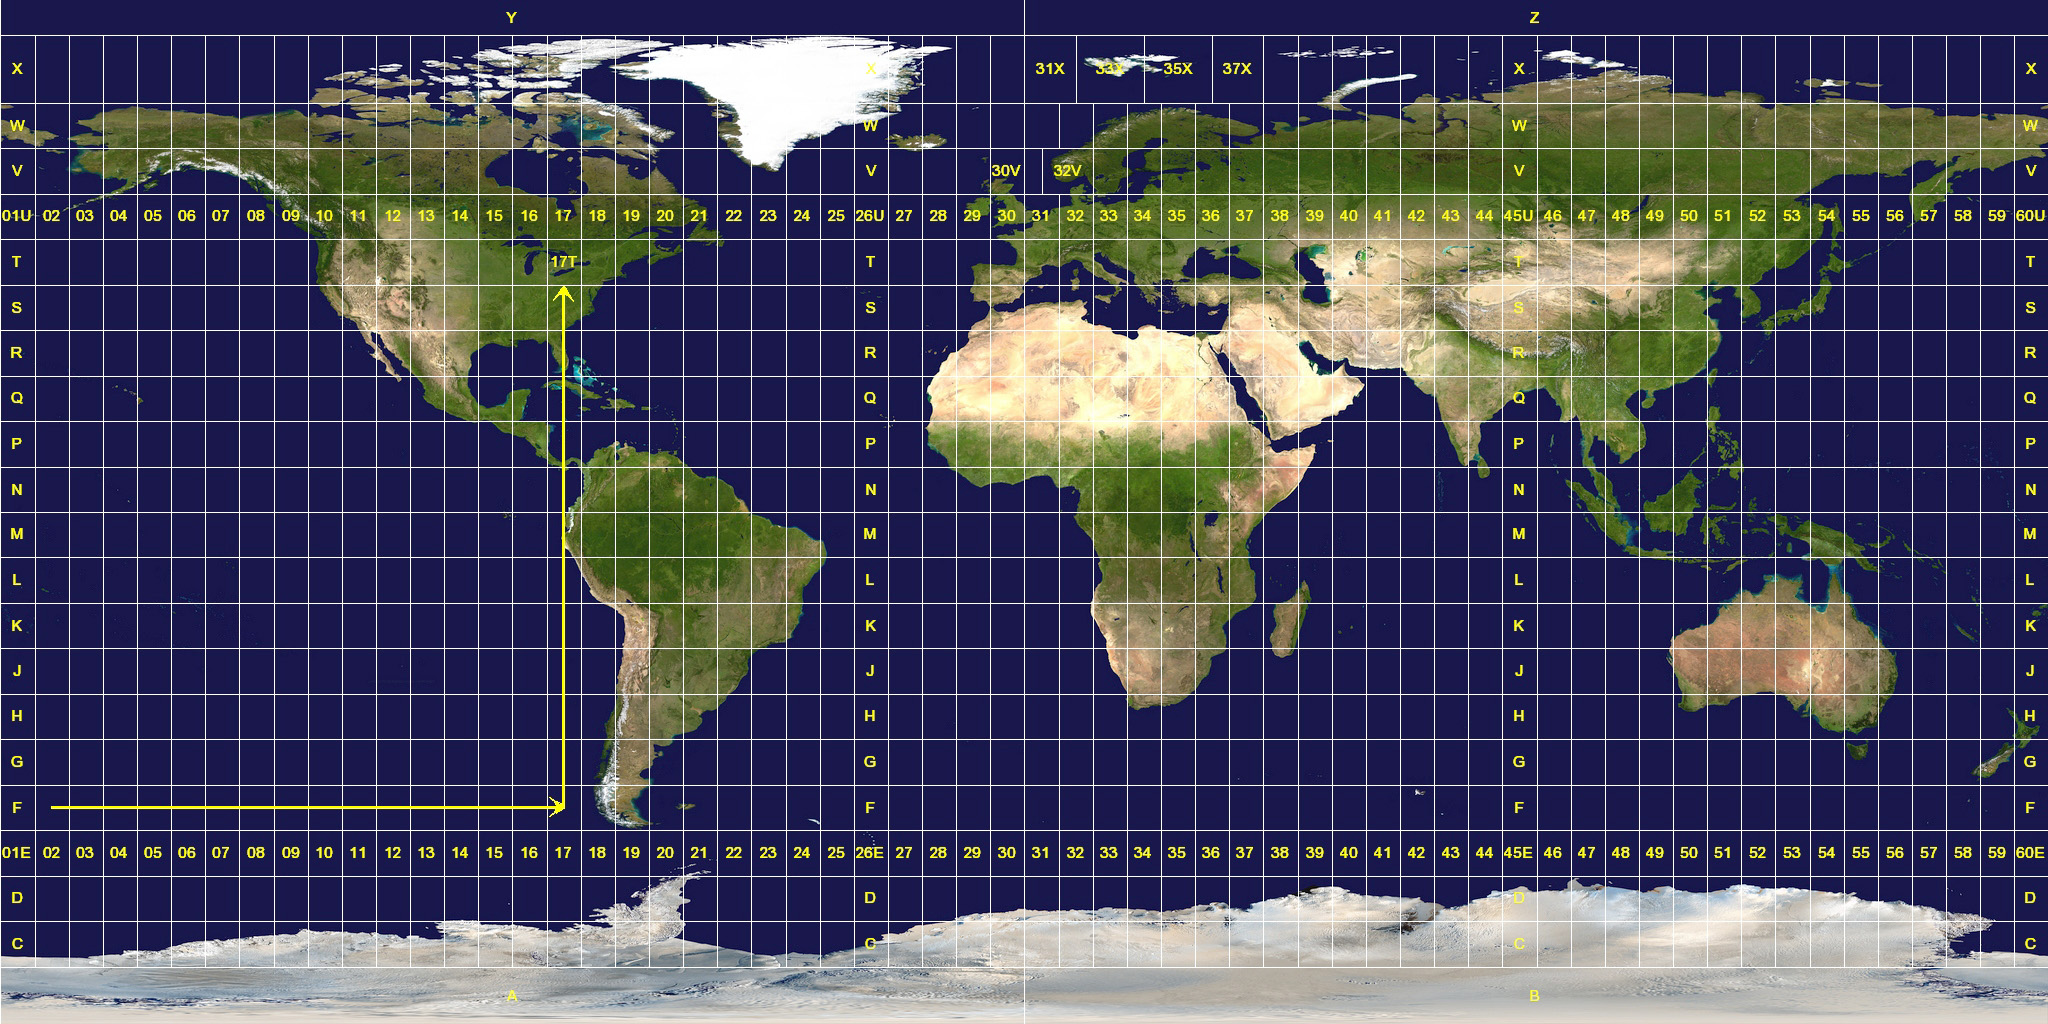
\includegraphics[width=\textwidth]{06.radionavegacion/Imagenes/Utm-zones.jpg}
  \caption{Zonas UTM}
  \label{fig:zonas.utm}
\end{figure}

Qué es el Datum de las coordenadas geográficas y su uso en el GPS
\url{https://www.aristasur.com/contenido/que-es-el-datum-de-las-coordenadas-geograficas-y-su-uso-en-el-gps}

\url{http://www.creaf.uab.es/master/intranet/MaterialsProfessors/PrincipisCartografia/MiquelNinyerola/Sistema_referencia_UTM_es.pdf}

\url{https://es.wikipedia.org/wiki/Sistema_de_coordenadas_universal_transversal_de_Mercator}